\chapter{RESULT AND ANALYSIS}
 \label{Chapter 5}
 \lhead{Chapter 5. \emph{Result \& Analysis}}
 

In this chapter, we aim to discuss the results of our implementation and analyze its performance in various scenarios and test setups.

\section{Evaluation Metrics}

\textbf{Classification Accuracy:}
Classification Accuracy is what we usually mean by the term accuracy. It is the highest used metric for classification tasks which works best when the number of samples belonging to each class is nearly equal. But, it does not convey any useful information when the dataset is imbalanced. For example, if any dataset has two classes: class A, and B, and 98\% of the dataset belongs to class A, blindly predicting each of the samples as class A will give an accuracy of 98\% which is misleading. Hence, this metric is only used in balanced datasets.
\begin{equation}
    Accuracy = \frac{\#\:correct\:predictions}{\#\:all\:samples}
\end{equation}

\textbf{Precision:}

precision is a measure of result relevancy, it calculates how many positive predictions are correct. It focuses on the correctness of positive detection which can be a good metric for cases where a false positive can be more troublesome than a false negative. 

\[ Precision = \frac{TP}{FP + TP}\]

\textbf{Recall:}
Unlike precision, Recall focuses on correctly identifying True Positives out of all the positive samples. It can be referred to it as Sensitivity or True Positive Rate.  It is a good metric where false negatives are more troublesome, such as in disease detection.

\[ Recall = \frac{TP}{FP + FN}\]

\textbf{F1 Score:}
It is a metric combination of both the Precision and Recall scores. It lets us do a tradeoff between Precision and Recall. A good F1 score is the indication of both good Recall and good Precision. That is why F1 score is considered one of the most important metrics to evaluate the performance of a classification system.

\[ F1\:Score = 2*\frac{Precision*Recall}{Precision + Recall}\]

\textbf{Area Under Curve (AUC):}
It is also known as AUC-ROC which signifies the area under the Receiver Operating Characteristic (ROC) curve. The ROC curve is an evaluation metric initially proposed for binary classification problems. In essence, it separates the "signal" from the "noise" by plotting the TPR against the FPR at different threshold values. The higher the AUC, the model is considered to perform better. In general, the ROC is for many different levels of thresholds and thus it has many F score values. F1 score is applicable for any particular point on the ROC curve.

\begin{figure}[H]
\centering
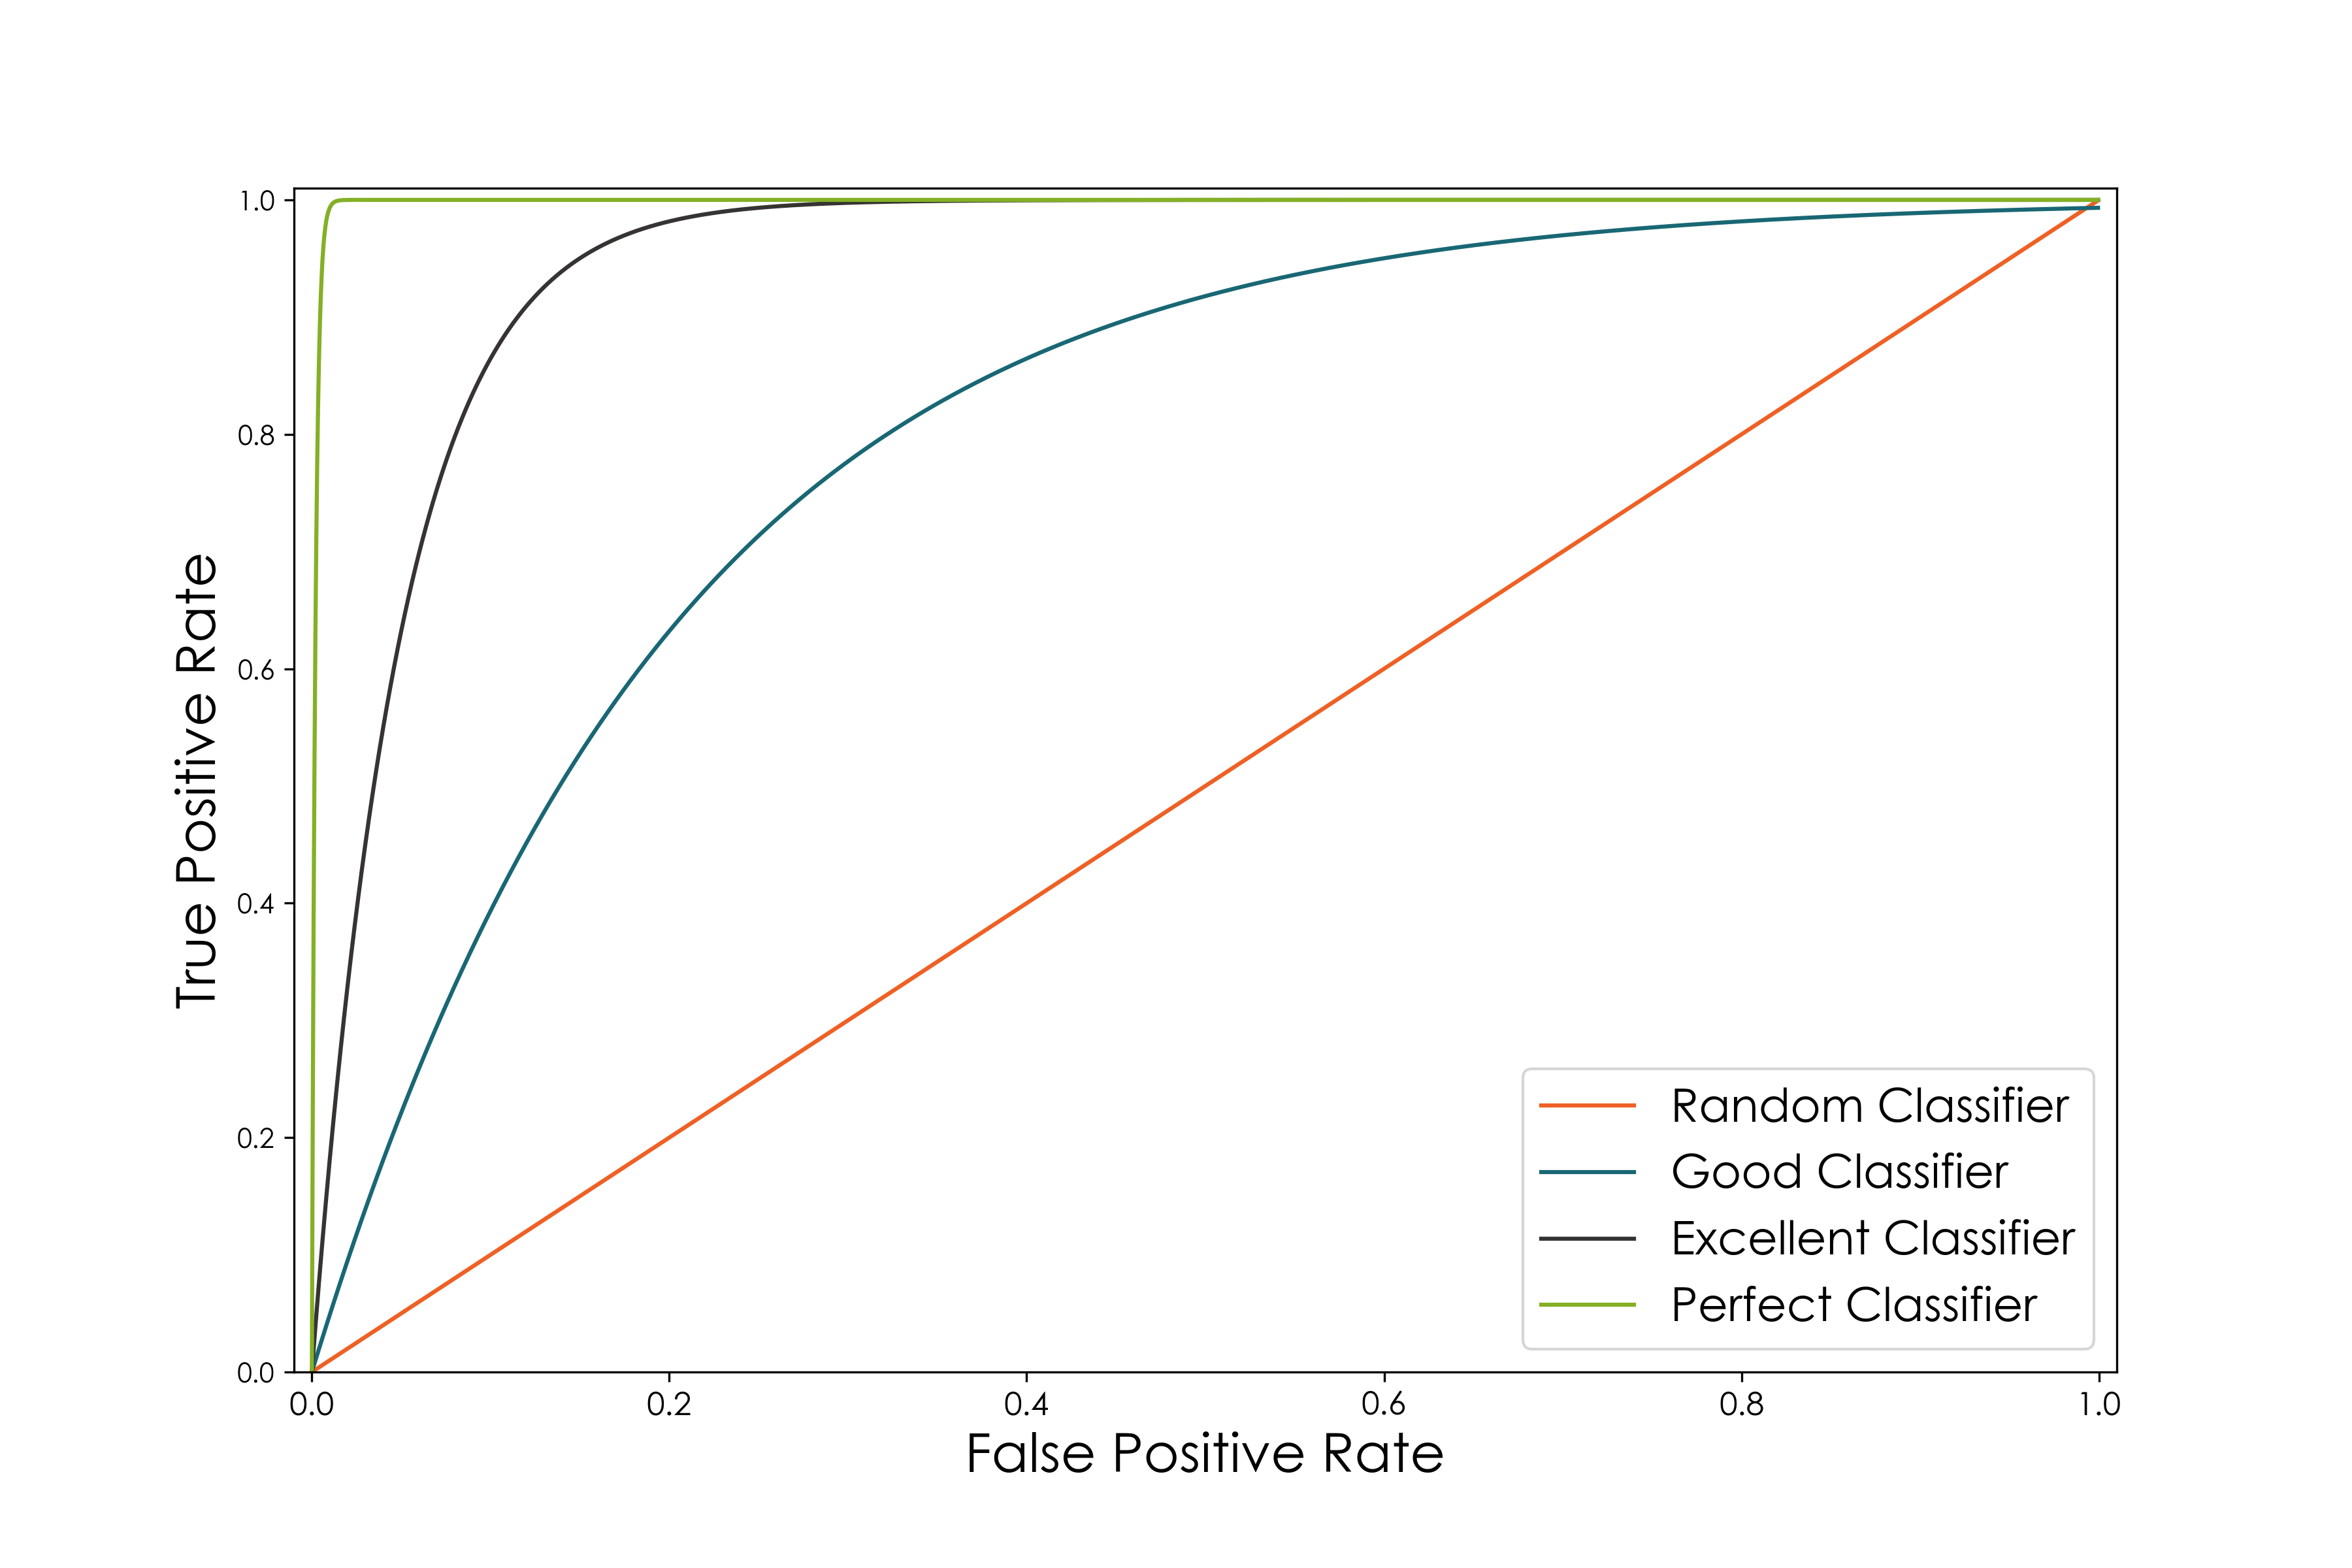
\includegraphics[width=1.0\textwidth]{./figure/chap 5/AUC.png}
\caption{Area Under Curve of Receiver Operating Characteristic (AUC-ROC)}
\label{Fig 5.1}
\end{figure}

\section{Testing Setups}
The prerequisite for building a good machine learning model is to validate its performance of it against unknown data. If not, the model may \emph{overfit} on the given dataset and perform worse in the actual application where we test the model on real-life unknown data. To do so, we generally split the dataset into some sets which are typically known as training set, testing set and so on. The model should not only work well on the training data but also give an accurate prediction on an unknown dataset. To evaluate how well the model is performing on unknown dataset, we employ different splitting techniques for better generalization.

\subsection{Train-test Split}
This is the most common type of the data splitting methods. In this method, we generally divide the dataset into two mutually exclusive sets. One is training set which is used to train the model and includes all the known labels. Another is testing set in which we hide the labels from the model and evaluate how does the model perform on unknown data. The split ratio is a term that defines how much data are in the training set and testing set. A split ratio of 75\% means 75\% of the total data are kept in training set and the rest 25\% data are in testing set. The split ratio is typically chosen between 60\% to 80\%, but a split ratio outside this range may be picked depending on the dataset. Generally, the split ratio keeps increasing with the dataset size.

\begin{figure}[H]
\centering
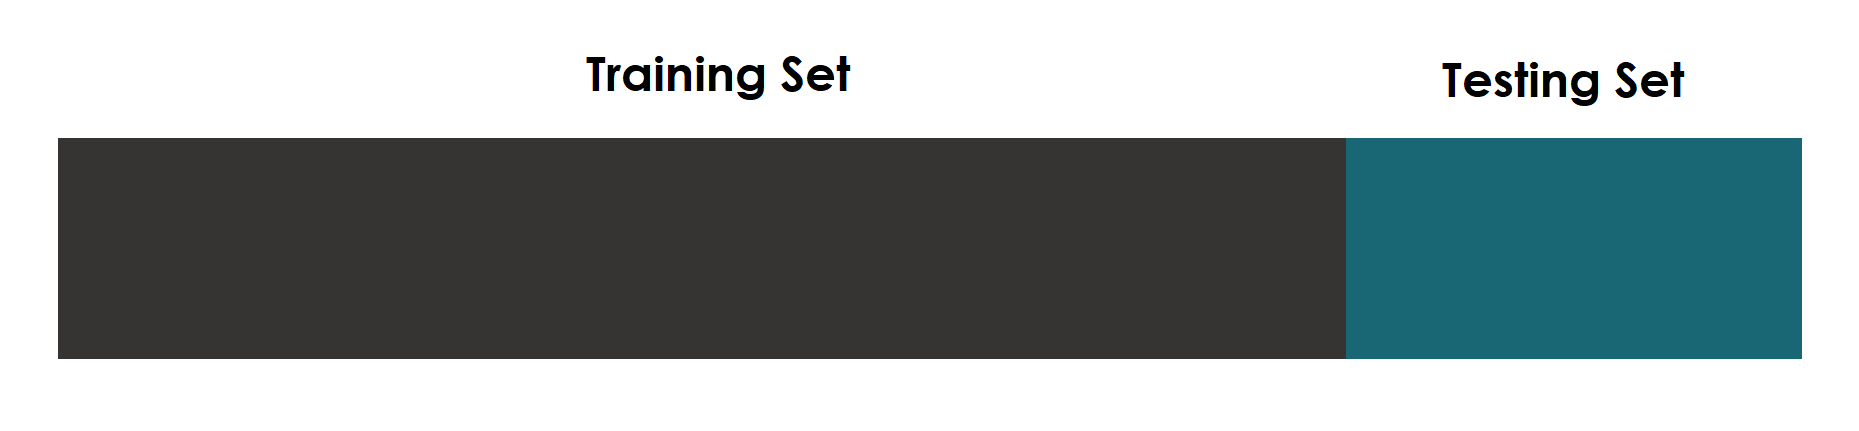
\includegraphics[width=1.0\textwidth]{./figure/chap 5/Train_test_split.png}
\caption{Train-test split}
\label{Fig 5.2}
\end{figure}

\subsection{Train-validation-test Split}
Sometimes the dataset is divided into three sets instead of two, adding another set known as validation set. This splitting technique is called train-validation-test split. In such a case, the data is first trained on training set and validated on the validation set to evaluate the performance. The model that has the best performance on the validation set is chosen and is tested on the testing set to obtain the actual performance of the model. 

\begin{figure}[H]
\centering
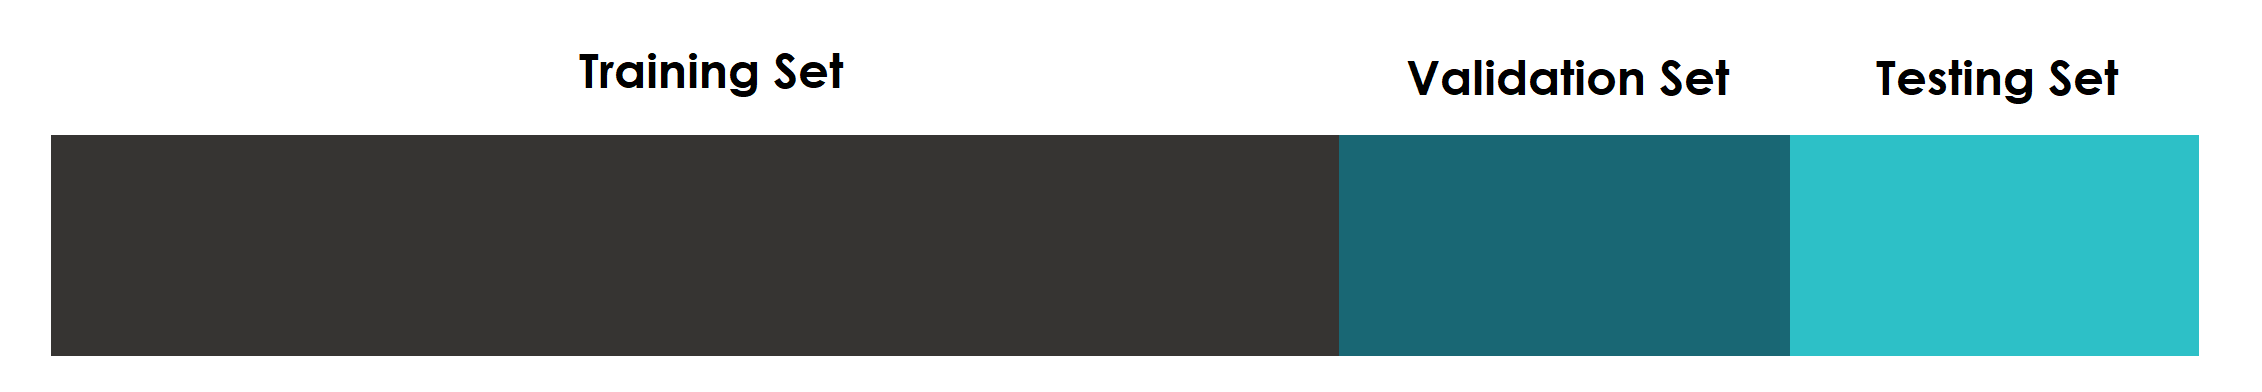
\includegraphics[width=1.0\textwidth]{./figure/chap 5/Train_val_test_split.png}
\caption{Train-validation-test split}
\label{Fig 5.3}
\end{figure}

\subsection{K-fold Cross Validation}
Cross-validation is a statistical splitting method used to estimate the skill of machine learning models. The procedure has a single parameter called $k$ which signifies how many splits will be made. When a particular number for k is selected, it may be substituted for k in the model's reference, such as when k=10 is used to refer to 10-fold cross-validation. 
The general procedure of this method is given below:
\begin{enumerate}
    \item Randomly shuffle the dataset.
    \item Create $k$ groups from the dataset.
    \item For every distinct group:
    \begin{enumerate}
        \item The group should be used as a holdout or test data set.
        \item Use the remaining groupings as the training data set.
        \item Fit the model to the training data, then assess it against the test data.
    \end{enumerate}
    \item Repeat the procedure for $k$ times.
    \item Using a model evaluation metric, summarize the model's skill. 
\end{enumerate}

By following this procedure k-fold cross validation removes the splitting bias which is present in the previous techniques. 

\begin{figure}[H]
\centering
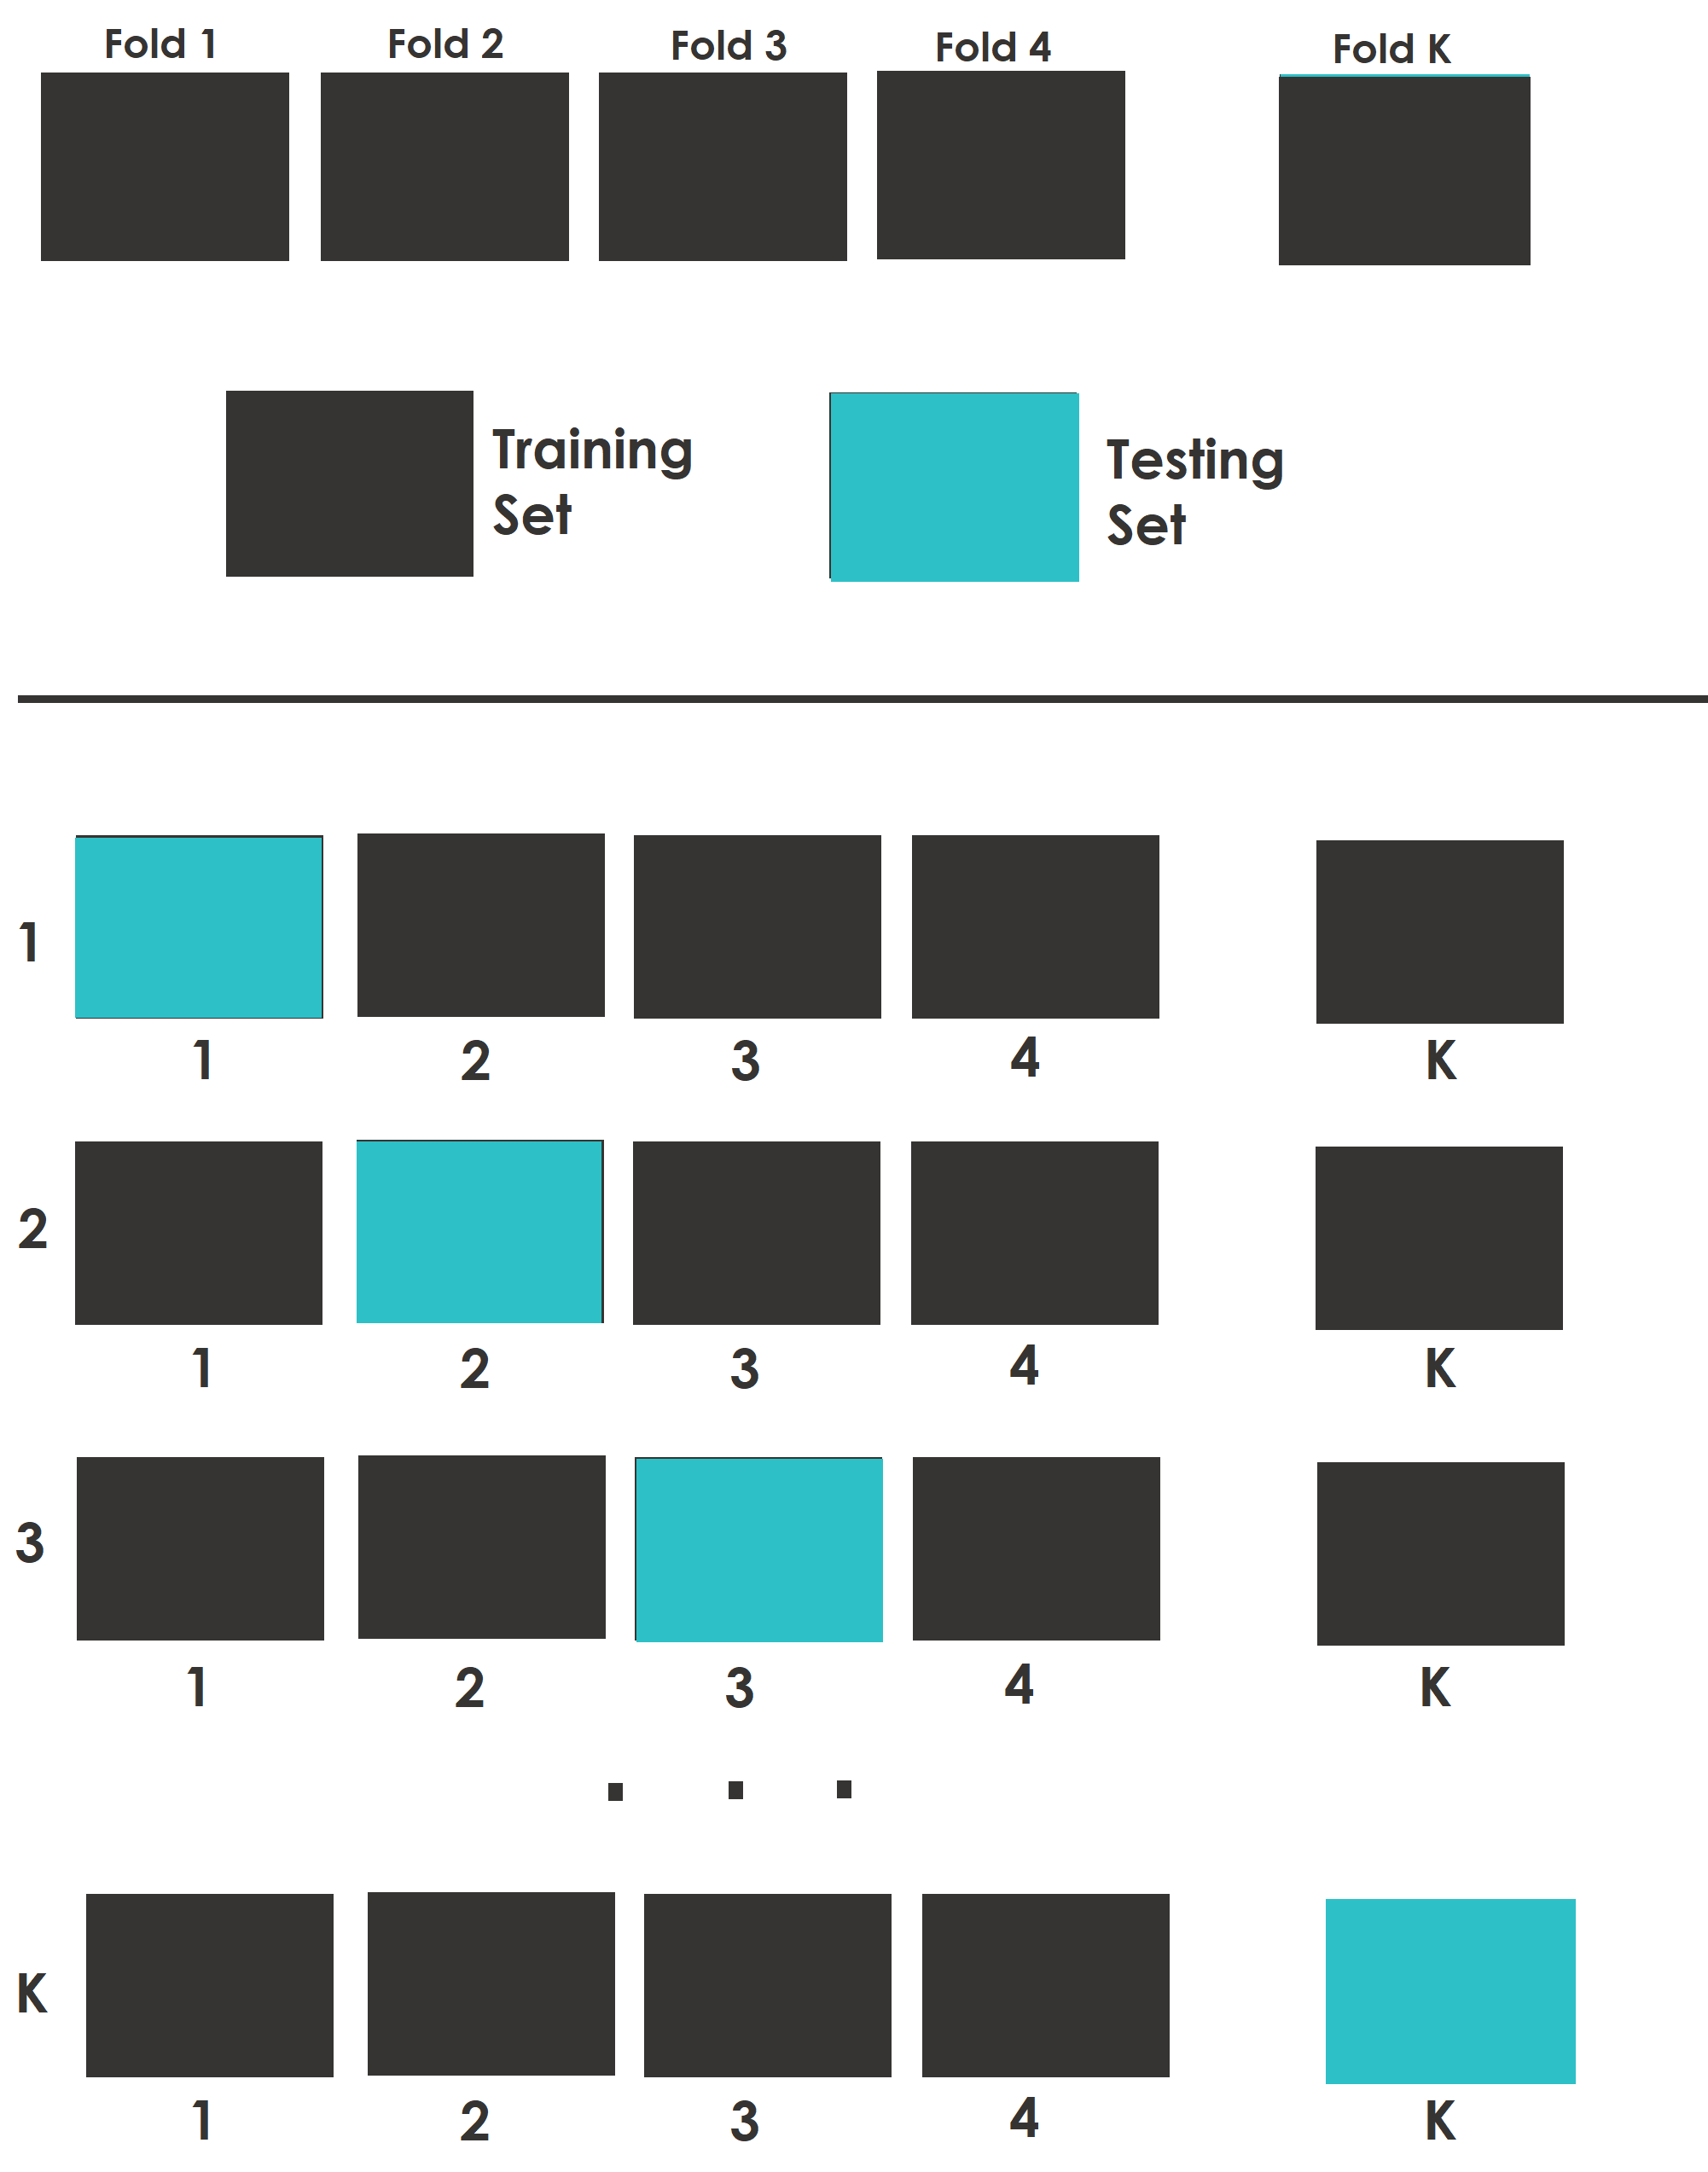
\includegraphics[width=0.8\textwidth]{./figure/chap 5/kfold.png}
\caption{K-fold cross validation}
\label{Fig 5.4}
\end{figure}


\subsection{Leave-One-Out Cross Validation (LOOCV)}
LOOCV is specially used in datasets where data are related to human subjects like in this dataset of human activity recognition. Different subjects carry out different activities in unique ways. Because of this variation, it is harder to predict a new subject's activity. To address this problem, we split the data according to each subject. That means each split contains only one subject's data. Then we perform the cross validation to assess the performance of the model on a new subject.

\section{Results}

\subsection{Fall Detection}
For the fall detection task, we had two classes: fall and non-fall. We experimented with different models and conducted a thorough hyperparameter tuning. Then we evaluated the performance of the models using a 75\% train-test split and a 10-fold cross validation. 
\begin{table}[H]
\caption{Result of fall detection}
\vspace{2mm}
\centering
\begin{tabular}{|c|cc|cc|}
\hline
\multirow{2}{*}{Model}    & \multicolumn{2}{c|}{75\% Train-test split}     & \multicolumn{2}{c|}{10-fold CV}          \\ \cline{2-5} 
                          & \multicolumn{1}{c|}{Accuracy} & F1 score & \multicolumn{1}{c|}{Accuracy} & F1 score \\ \hline
Logistic Regression       & \multicolumn{1}{c|}{0.657}    & 0.632    & \multicolumn{1}{c|}{0.762}    & 0.772    \\
Support Vector Classifier & \multicolumn{1}{c|}{0.938}    & 0.929    & \multicolumn{1}{c|}{0.921}    & 0.922    \\
K Nearest Neighbors       & \multicolumn{1}{c|}{0.923}    & 0.909    & \multicolumn{1}{c|}{0.921}    & 0.924    \\
Random Forest             & \multicolumn{1}{c|}{0.966}    & 0.962    & \multicolumn{1}{c|}{0.967}    & 0.967    \\
Extra Trees               & \multicolumn{1}{c|}{0.980}    & 0.978    & \multicolumn{1}{c|}{0.985}    & 0.985    \\
XGBoost                   & \multicolumn{1}{c|}{0.953}    & 0.947    & \multicolumn{1}{c|}{0.954}    & 0.959    \\ \hline
\end{tabular}
\label{Table 5.1}
\end{table}

Using the \ref{Table 5.1}, we can find the best model is the Extra Trees Classifier which obtained 98.5\% accuracy and F1 score in 10-fold CV and 98\% and 97.8\% accuracy and F1 score in 75\% train-test split. We plotted the confusion matrix of this model for 75\% train-test split.

\begin{figure}[H]
\centering
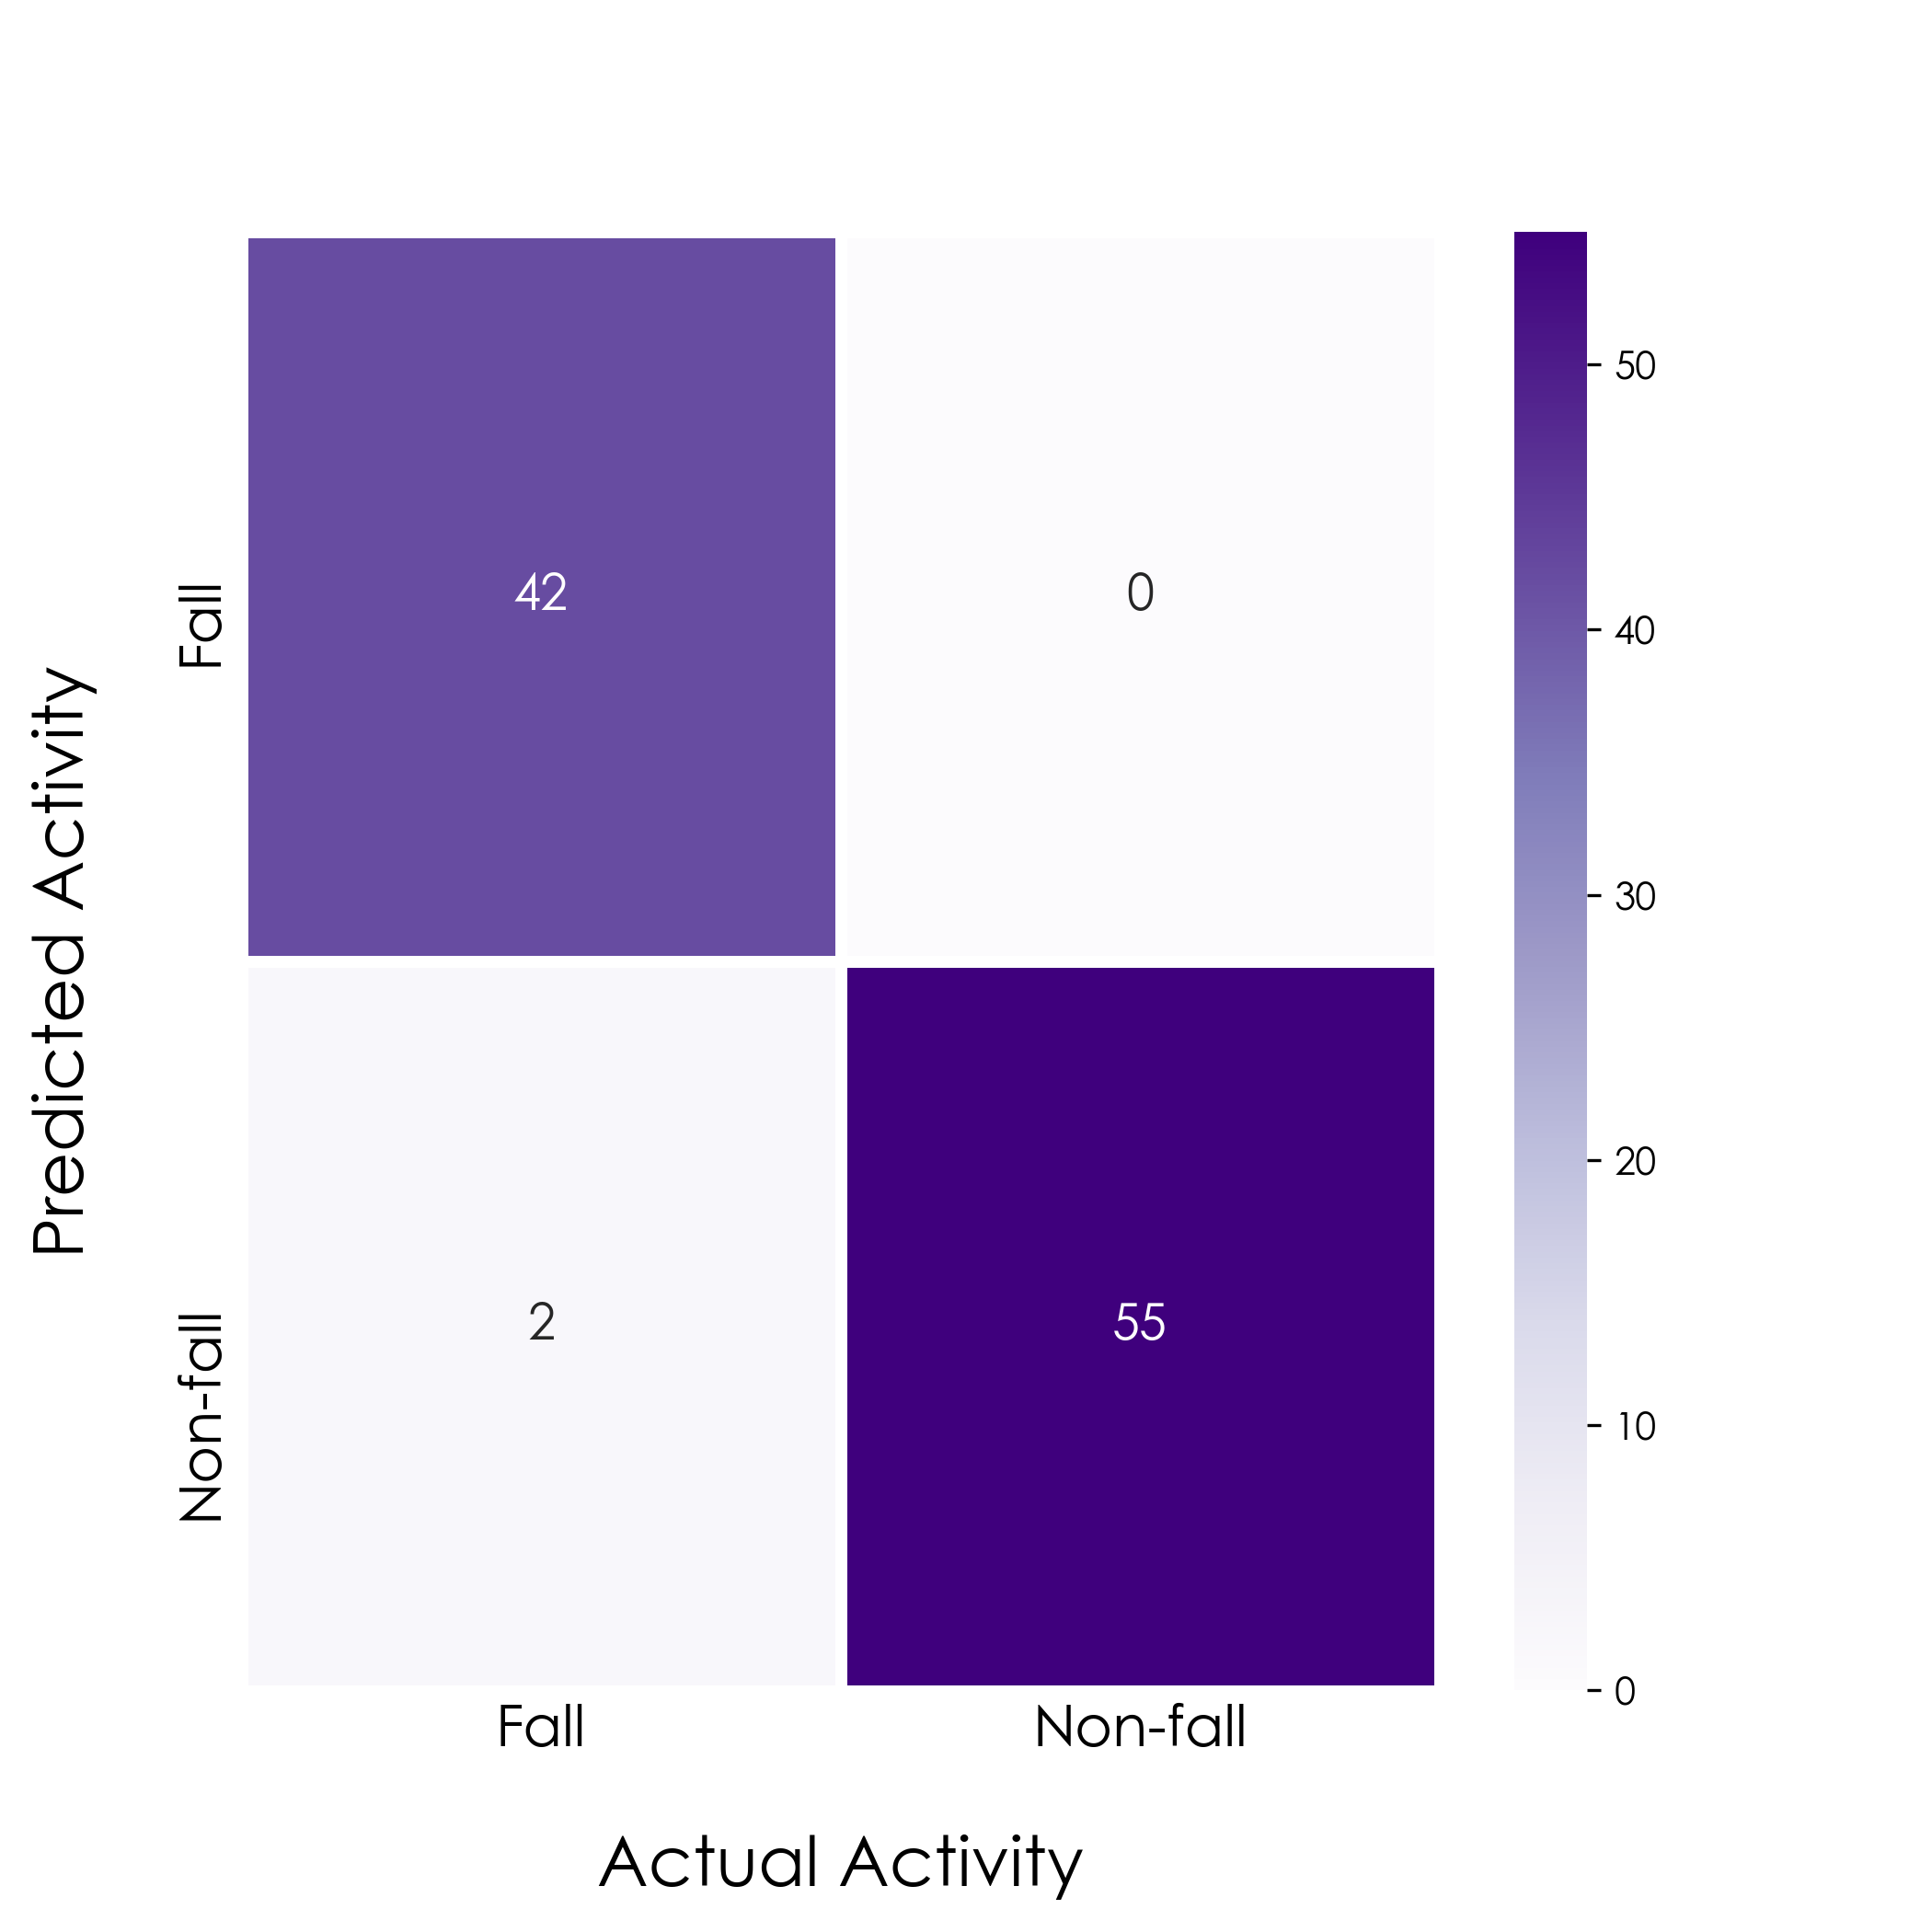
\includegraphics[width=1\textwidth]{./figure/chap 5/conf_binary.png}
\caption{Confusion matrix for fall detection}
\label{Fig 5.5}
\end{figure}

The results of fall detection is summarized in \ref{Fig 5.6}
\begin{figure}[H]
\centering
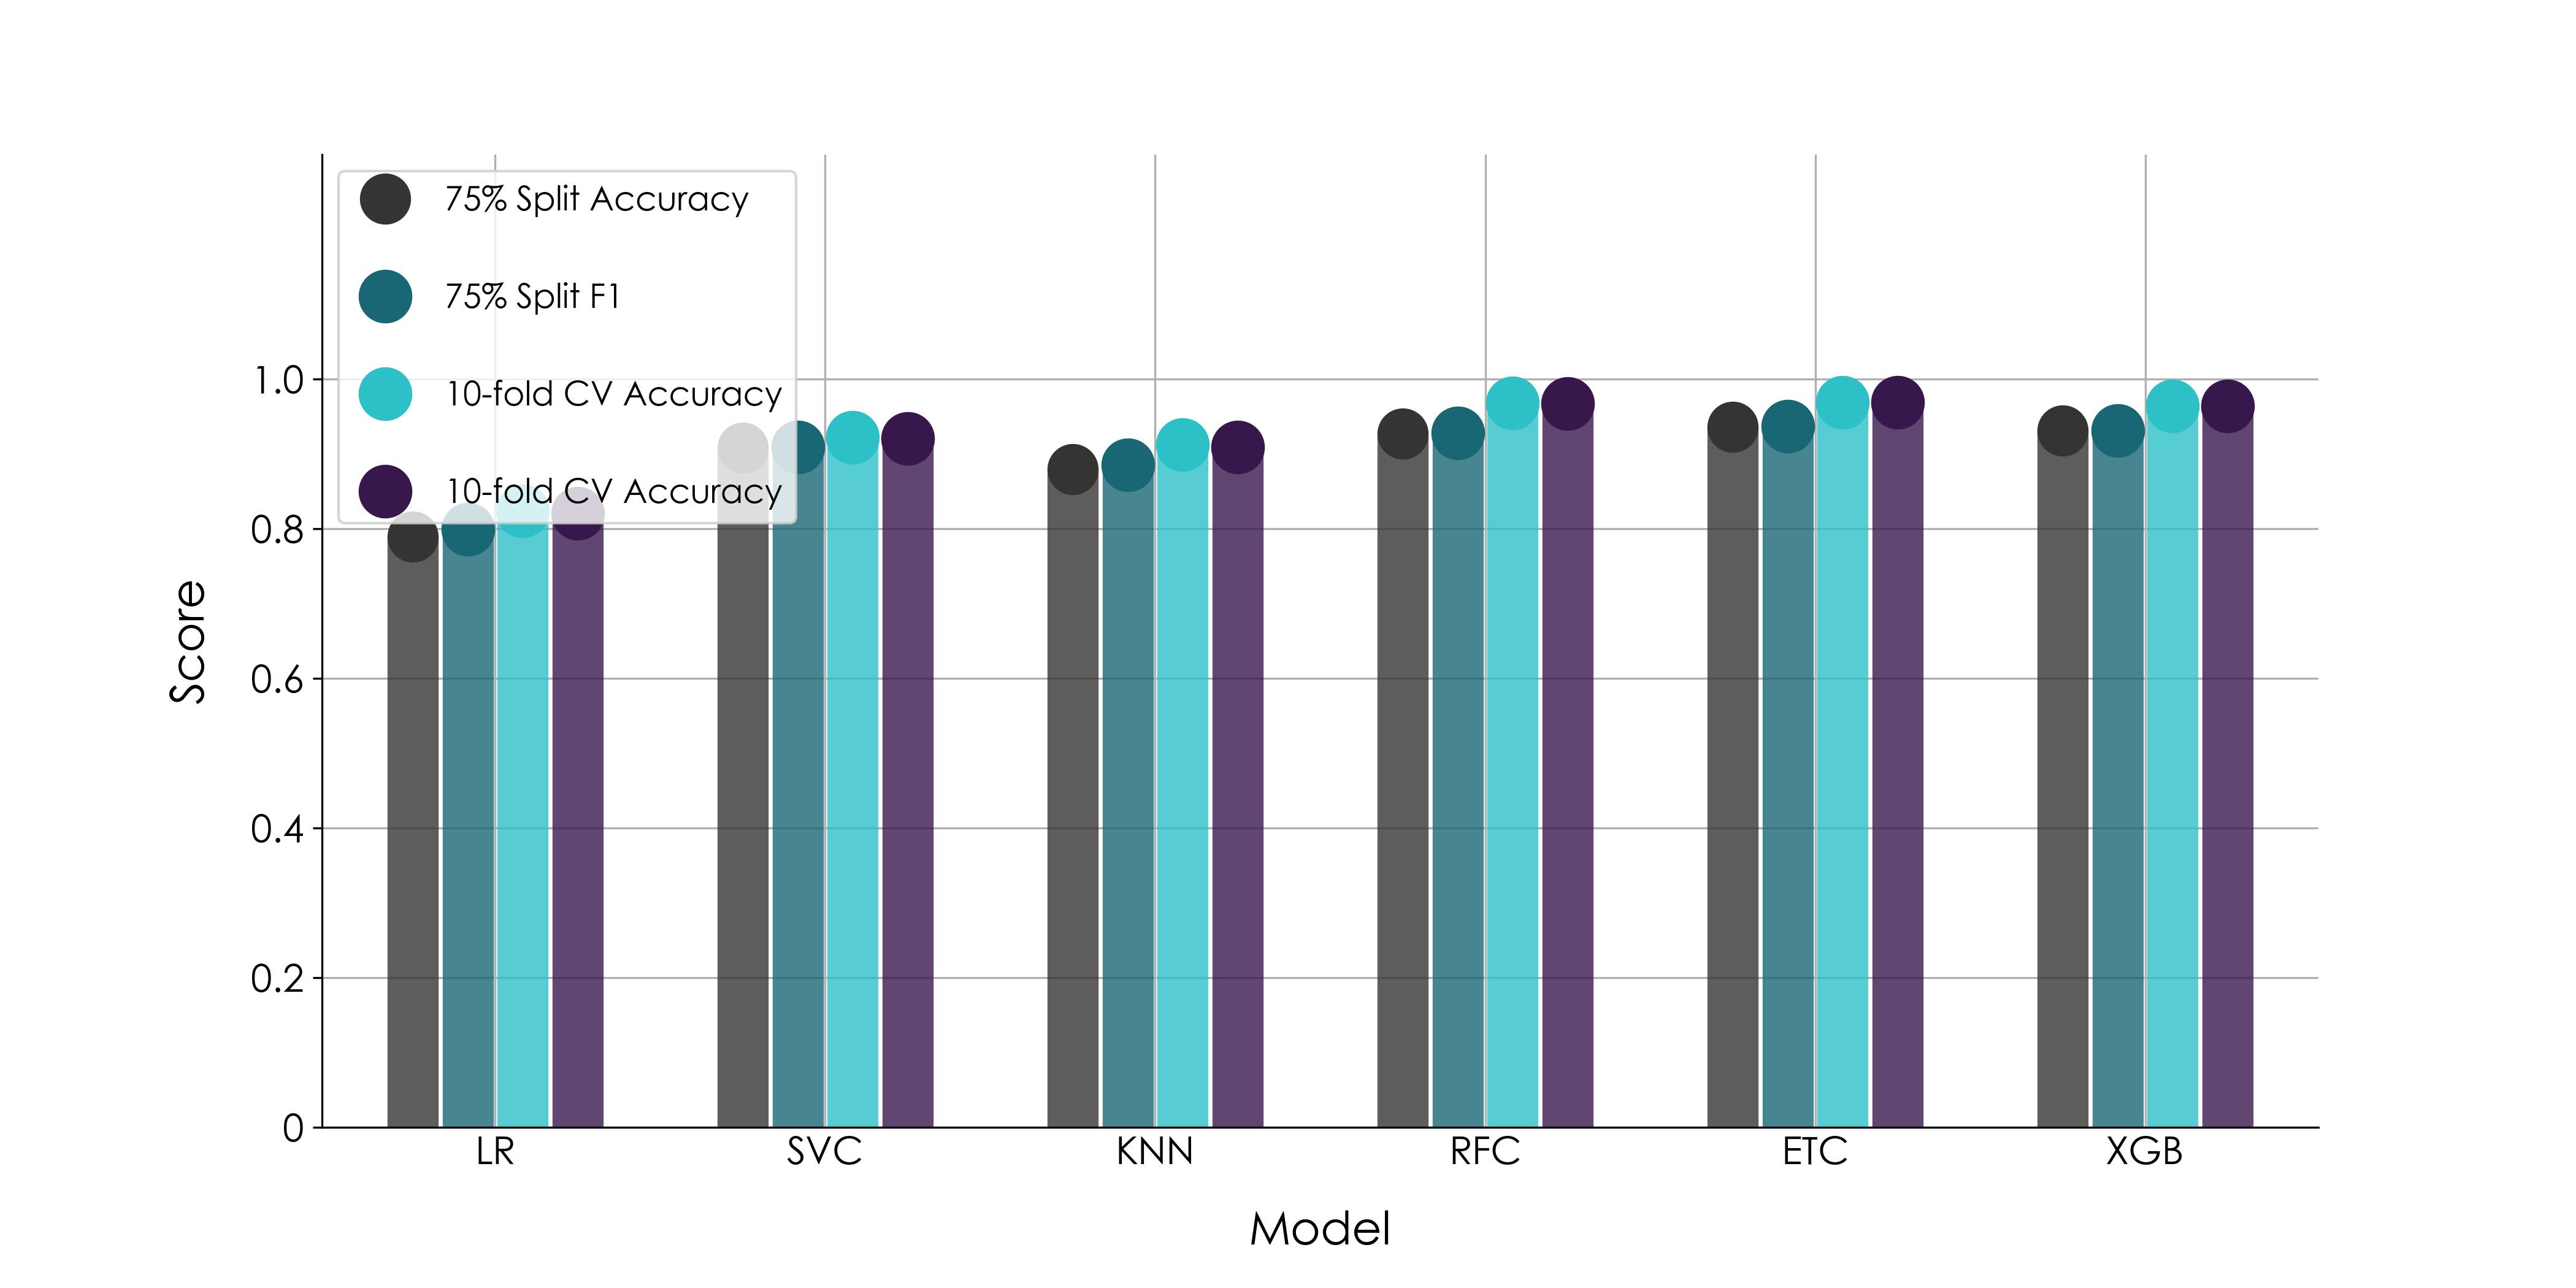
\includegraphics[width=1\textwidth]{./figure/chap 5/binary_model_scores.png}
\caption{Fall detection results}
\label{Fig 5.6}
\end{figure}

\subsection{Human Activity Recognition}
We have five classes of human activity: fall, walk, stand, empty room and presence. We took a similar approach for human activity recognition as fall detection mentioned in the previous sub-section. The results are depicted in table \ref{Table 5.2}.

\begin{table}[H]
\caption{Result of human activity recognition}
\vspace{2mm}
\centering
\begin{tabular}{|c|cc|cc|}
\hline
\multirow{2}{*}{Model}    & \multicolumn{2}{c|}{75\% Train-test split}     & \multicolumn{2}{c|}{10-fold CV}          \\ \cline{2-5} 
                          & \multicolumn{1}{c|}{Accuracy} & F1 score & \multicolumn{1}{c|}{Accuracy} & F1 score \\ \hline
Logistic Regression       & \multicolumn{1}{c|}{0.789}    & 0.799    & \multicolumn{1}{c|}{0.824}    & 0.82     \\
Support Vector Classifier & \multicolumn{1}{c|}{0.908}    & 0.909    & \multicolumn{1}{c|}{0.922}    & 0.92     \\
K Nearest Neighbors       & \multicolumn{1}{c|}{0.879}    & 0.885    & \multicolumn{1}{c|}{0.912}    & 0.909    \\
Random Forest             & \multicolumn{1}{c|}{0.927}    & 0.928    & \multicolumn{1}{c|}{0.968}    & 0.967    \\
Extra Trees               & \multicolumn{1}{c|}{0.936}    & 0.937    & \multicolumn{1}{c|}{0.969}    & 0.969    \\
XGBoost                   & \multicolumn{1}{c|}{0.931}    & 0.931    & \multicolumn{1}{c|}{0.964}    & 0.964    \\ \hline
\end{tabular}
\label{Table 5.2}
\end{table}

Like fall detection, the Extra Trees Classifier gives better results in this task too. The obtained confusion matrix is shown in \ref{Fig 5.7}.

\begin{figure}[H]
\centering
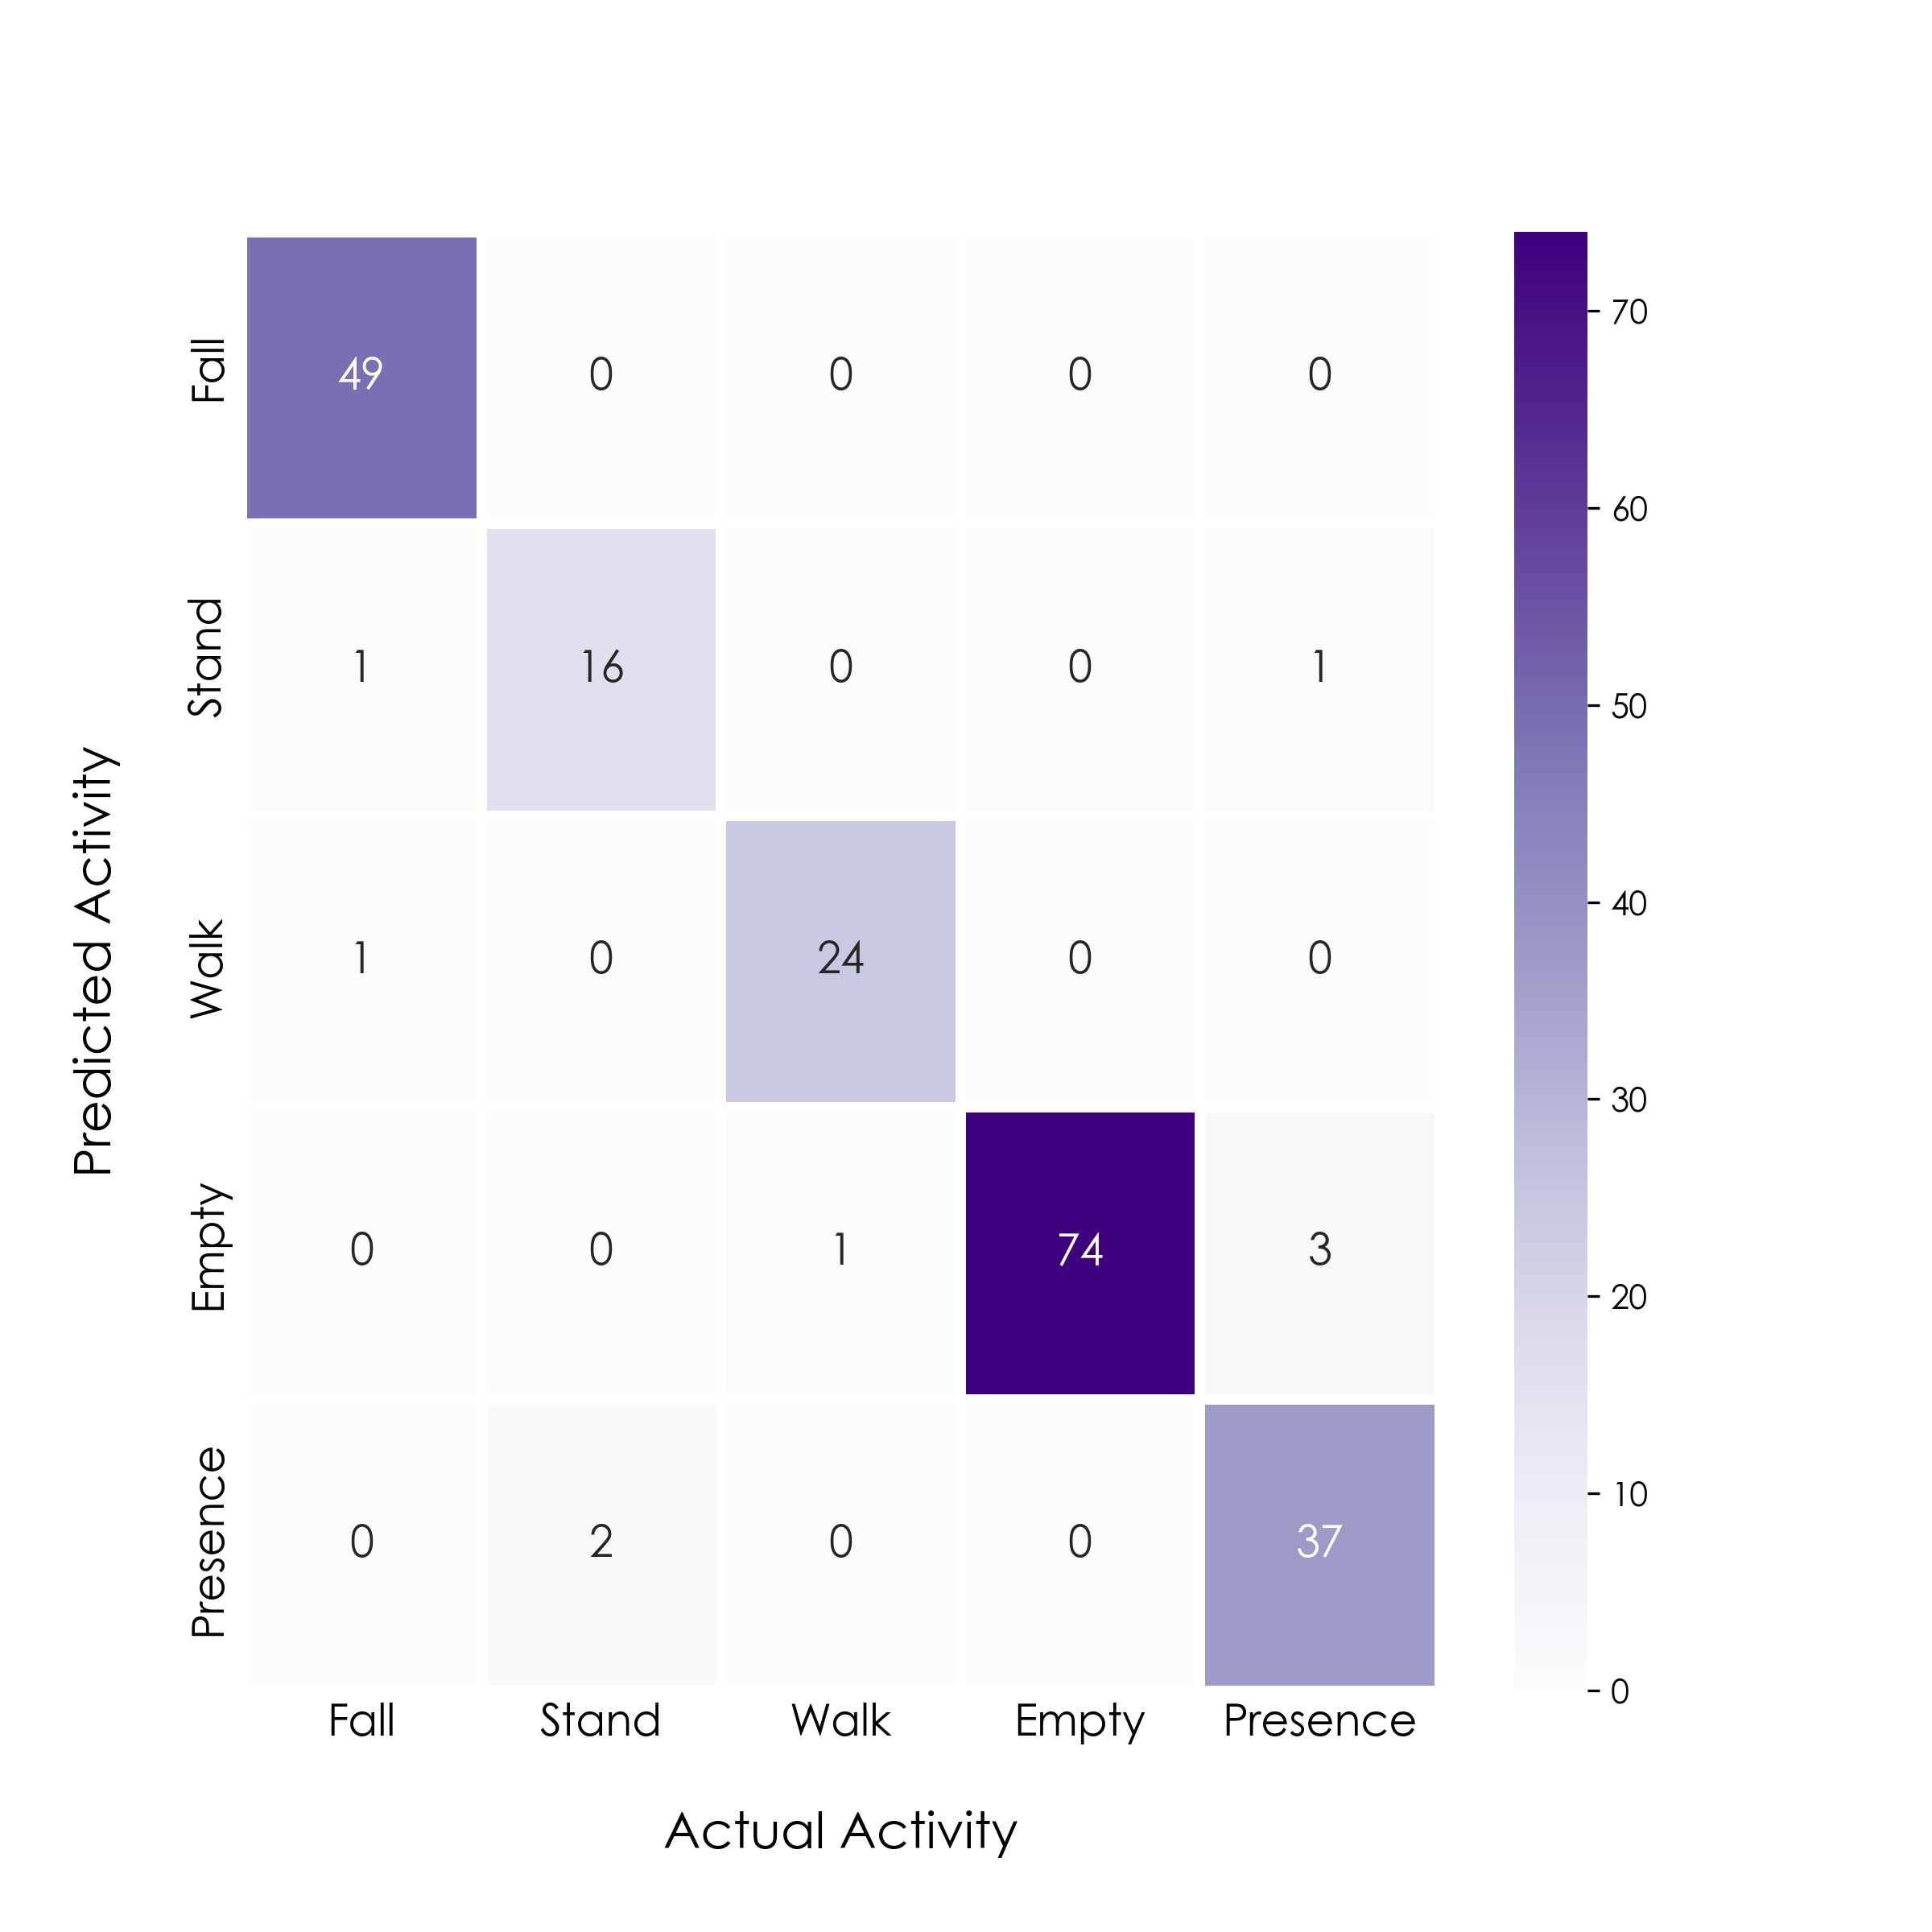
\includegraphics[width=1\textwidth]{./figure/chap 5/conf_multiclass.png}
\caption{Confusion matrix for human activity recognition}
\label{Fig 5.7}
\end{figure}

The results of human activity recognition is summarized in \ref{Fig 5.8}
\begin{figure}[H]
\centering
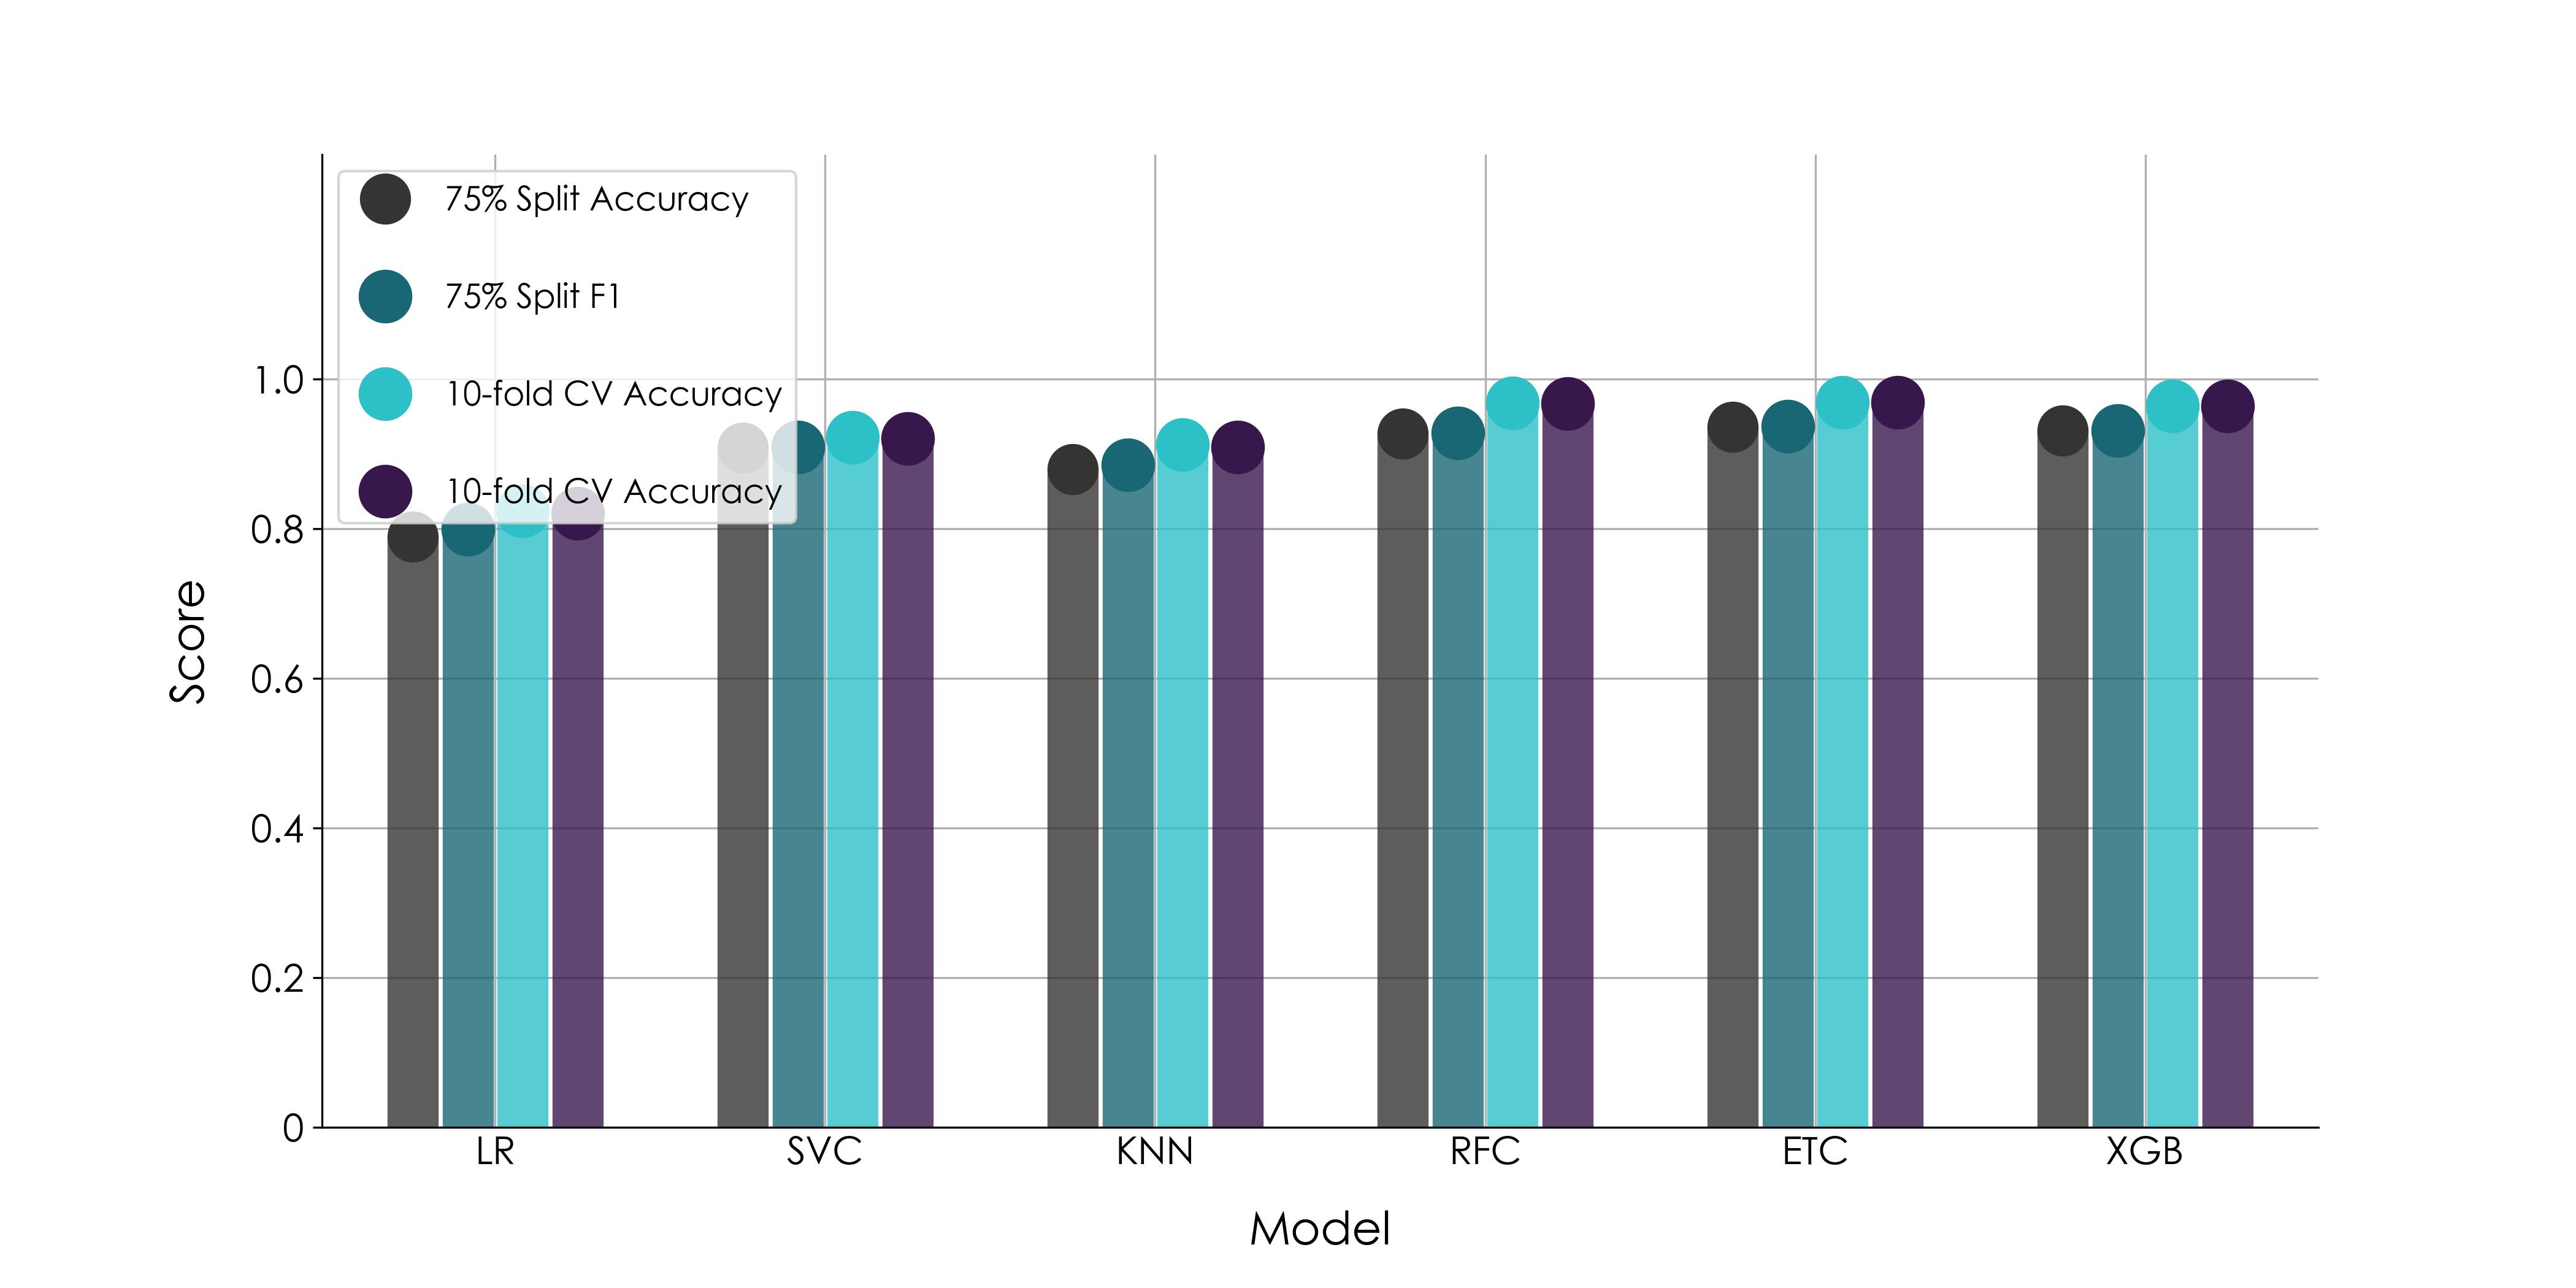
\includegraphics[width=1\textwidth]{./figure/chap 5/multiclass_model_scores.png}
\caption{Human activity recognition results}
\label{Fig 5.8}
\end{figure}

\section{Analysis of in Terms of Speed}
We also conducted an execution time analysis to show that our proposed system is able to run in real-time. The analysis was done on a total of 400 data samples where 300 of them were in the training set and the remaining 100 data samples were in the test set. So, the training data collection time was 1200 seconds and the test data collection time was 400 seconds. We used a lower mid-level laptop with core i5 7200U processor clocked at 2.5 GHz and 8GB RAM to run the time analysis. By looking at \ref{Table 5.3} we can see that, to process the inference data of 400 seconds, the best model Extra trees took only 5 seconds to predict in the multiclass classification problem and 4 seconds to predict in the binary classification problem. So, this system is capable of processing data from up to 80 devices simultaneously  in real-time. Also, the fastest model tested was K Nearest Neighbors which took only 0.1 seconds to predict a data of 400 seconds. So, it can easily be concluded that our proposed system can run and infer in real-time for a number of devices simultaneously.

% Please add the following required packages to your document preamble:
% \usepackage{multirow}
\begin{table}[H]
\caption{Execution time of the models}
\vspace{2mm}
\centering
\begin{tabular}{|c|cc|cc|}
\hline
\multirow{2}{*}{Model}    & \multicolumn{2}{c|}{Binary Classification}                                                                                                        & \multicolumn{2}{c|}{Multi-class Classification}                                                                                                   \\ \cline{2-5} 
                          & \multicolumn{1}{c|}{\begin{tabular}[c]{@{}c@{}}Training \\ time (s)\end{tabular}} & \begin{tabular}[c]{@{}c@{}}Inference \\ time (s)\end{tabular} & \multicolumn{1}{c|}{\begin{tabular}[c]{@{}c@{}}Training \\ time (s)\end{tabular}} & \begin{tabular}[c]{@{}c@{}}Inference \\ time (s)\end{tabular} \\ \hline
Logistic Regression       & \multicolumn{1}{c|}{1.4}                                                          & 0.2                                                           & \multicolumn{1}{c|}{1.6}                                                          & 0.2                                                           \\
Support Vector Classifier & \multicolumn{1}{c|}{2}                                                            & 0.2                                                           & \multicolumn{1}{c|}{2}                                                            & 0.2                                                           \\
K Nearest Neighbors       & \multicolumn{1}{c|}{0.3}                                                          & 0.1                                                           & \multicolumn{1}{c|}{0.4}                                                          & 0.1                                                           \\
Random Forest             & \multicolumn{1}{c|}{15}                                                           & 3                                                             & \multicolumn{1}{c|}{30}                                                           & 6                                                             \\
Extra Trees               & \multicolumn{1}{c|}{15}                                                           & 4                                                             & \multicolumn{1}{c|}{17}                                                           & 5                                                            \\
XGBoost                   & \multicolumn{1}{c|}{18}                                                           & 4                                                             & \multicolumn{1}{c|}{26}                                                           & 6                                                             \\ \hline
\end{tabular}
\label{Table 5.3}
\end{table}